\documentclass[12pt,letterpaper]{article}

\usepackage{amsmath, amsthm}
\usepackage{microtype, parskip}
\usepackage[comma,numbers,sort&compress]{natbib}
\usepackage{lineno}
\usepackage{docmute}
\usepackage{caption, subcaption, multirow, morefloats, rotating}
\usepackage{wrapfig}

\frenchspacing

\captionsetup[subfigure]{position = top, labelfont = bf, textfont = normalfont, singlelinecheck = off, justification = raggedright}

\begin{document}
\section{Results}

% Model fit
%   survival curve
%   deviance residuals
%   posterior predictive point tests
%   weibull > exponential (supported by WAIC)
As stated above, posterior approximations for both the exponential and Weibull models achieved approximate stationarity after approximately 10,000 steps as all parameter estimates have an \(\hat{R} < 1.1\) \uppercase{ref tables}. 

Comparisons of the survival functions estimated from 1000 posterior predictive estimated data sets to the estimated survival function of the observed genera demonstrates that both the exponential and Weibull models approximately capture the observed pattern of extinction (Fig. \ref{fig:surv}). The major difference in fit between the two models is that the Weibull model has a slightly better fit for longer lived taxa than the exponential model.

\begin{figure}[ht]
  \centering
  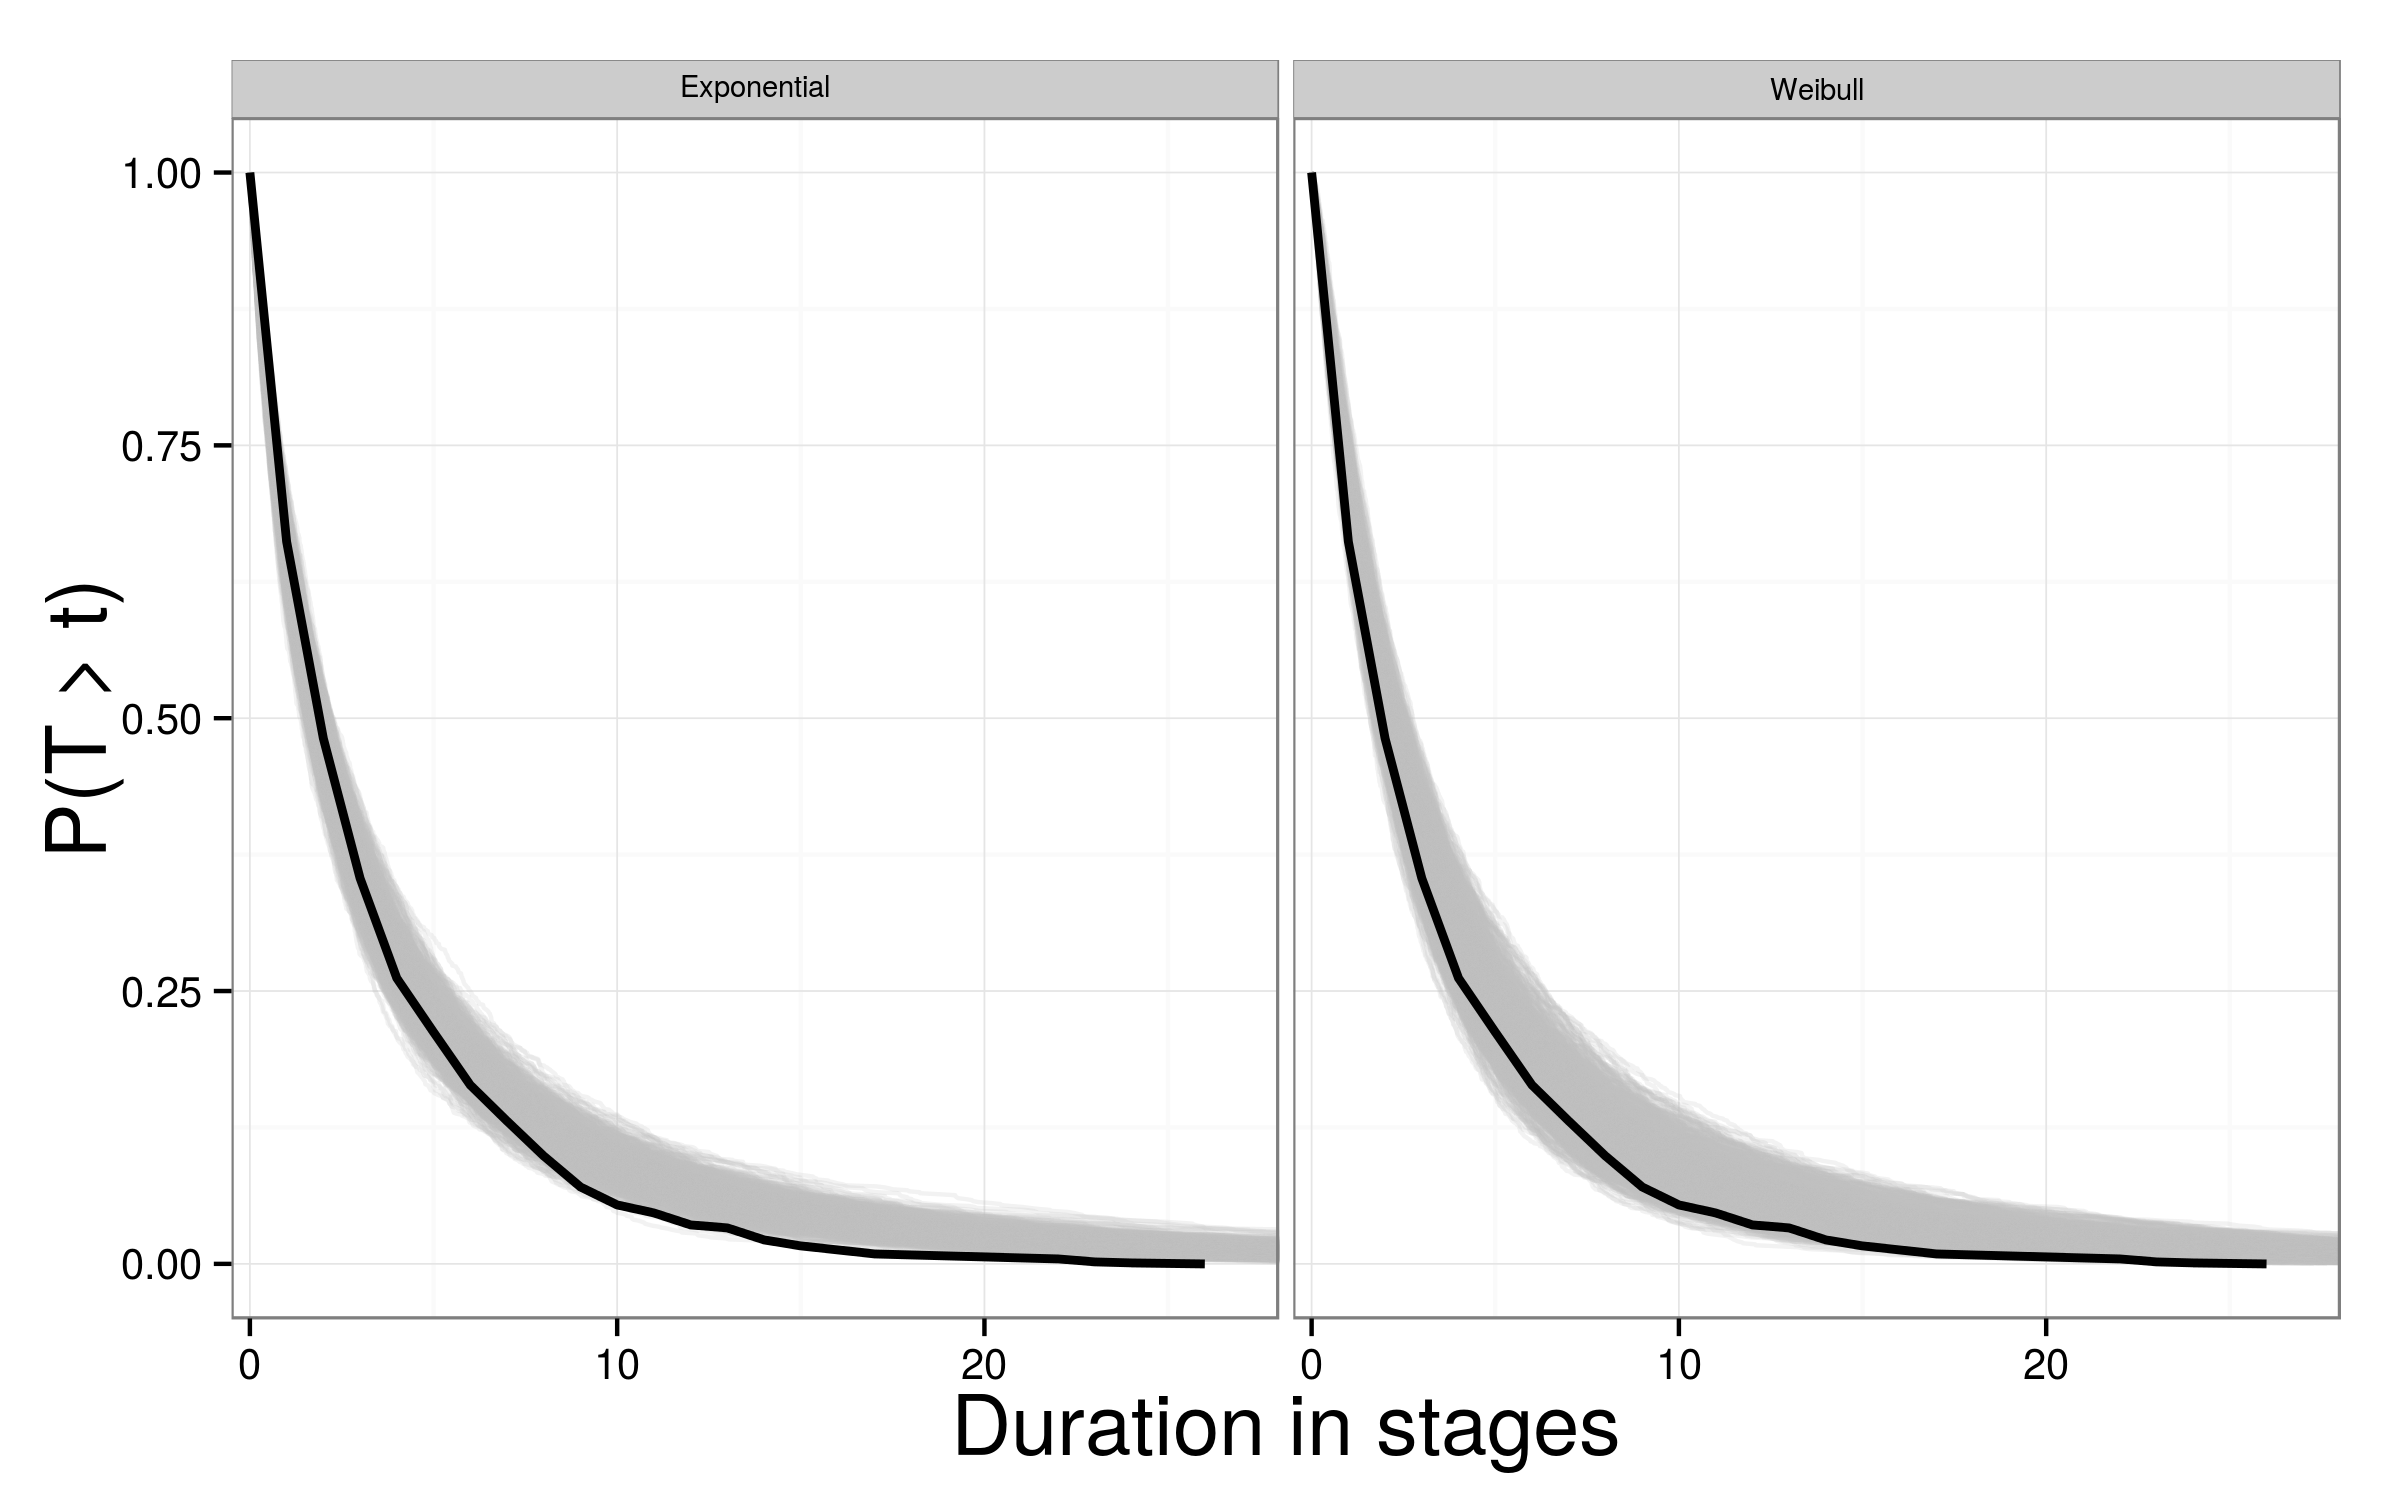
\includegraphics[height = 0.5\textheight,width=\textwidth,keepaspectratio=true]{figure/survival_curves}
  \caption{<+caption text+>}
  \label{fig:surv}
\end{figure}

Inspection of the deviance residuals yields a similar pattern of biased estimates for longer lived taxa \uppercase{ref figure}. 

Finally, the Weibull model is expected to have slightly better out-of-sample predictive accuracy when compared to the exponential model \uppercase{values}. This is congruent with graphical comparisons of the survival functions (Fig. \ref{fig:surv}). Because the difference between the WAIC scores is small, both results from the exponential and Weibull models will be analyzed.

% Results/hypothesis tests
%   \mu of hierarchical effects
%   \tau of hierarchical effects (partial pooling)
Estimates of the overall overall mean covariate effects \(\mu_{\mathbf{B}}\) can be considered time-invariant generalizations for brachiopod survival for the Paleozoic \uppercase{Smits in prep} (Fig. \ref{fig:mu}). Consistent with expectations, geographic range size has a negative effect on extinction risk where genera with large ranges having greater durations than genera with small ranges. I also find no time-invariant effect of body size on genus duration. 
\begin{figure}[ht]
  \centering
  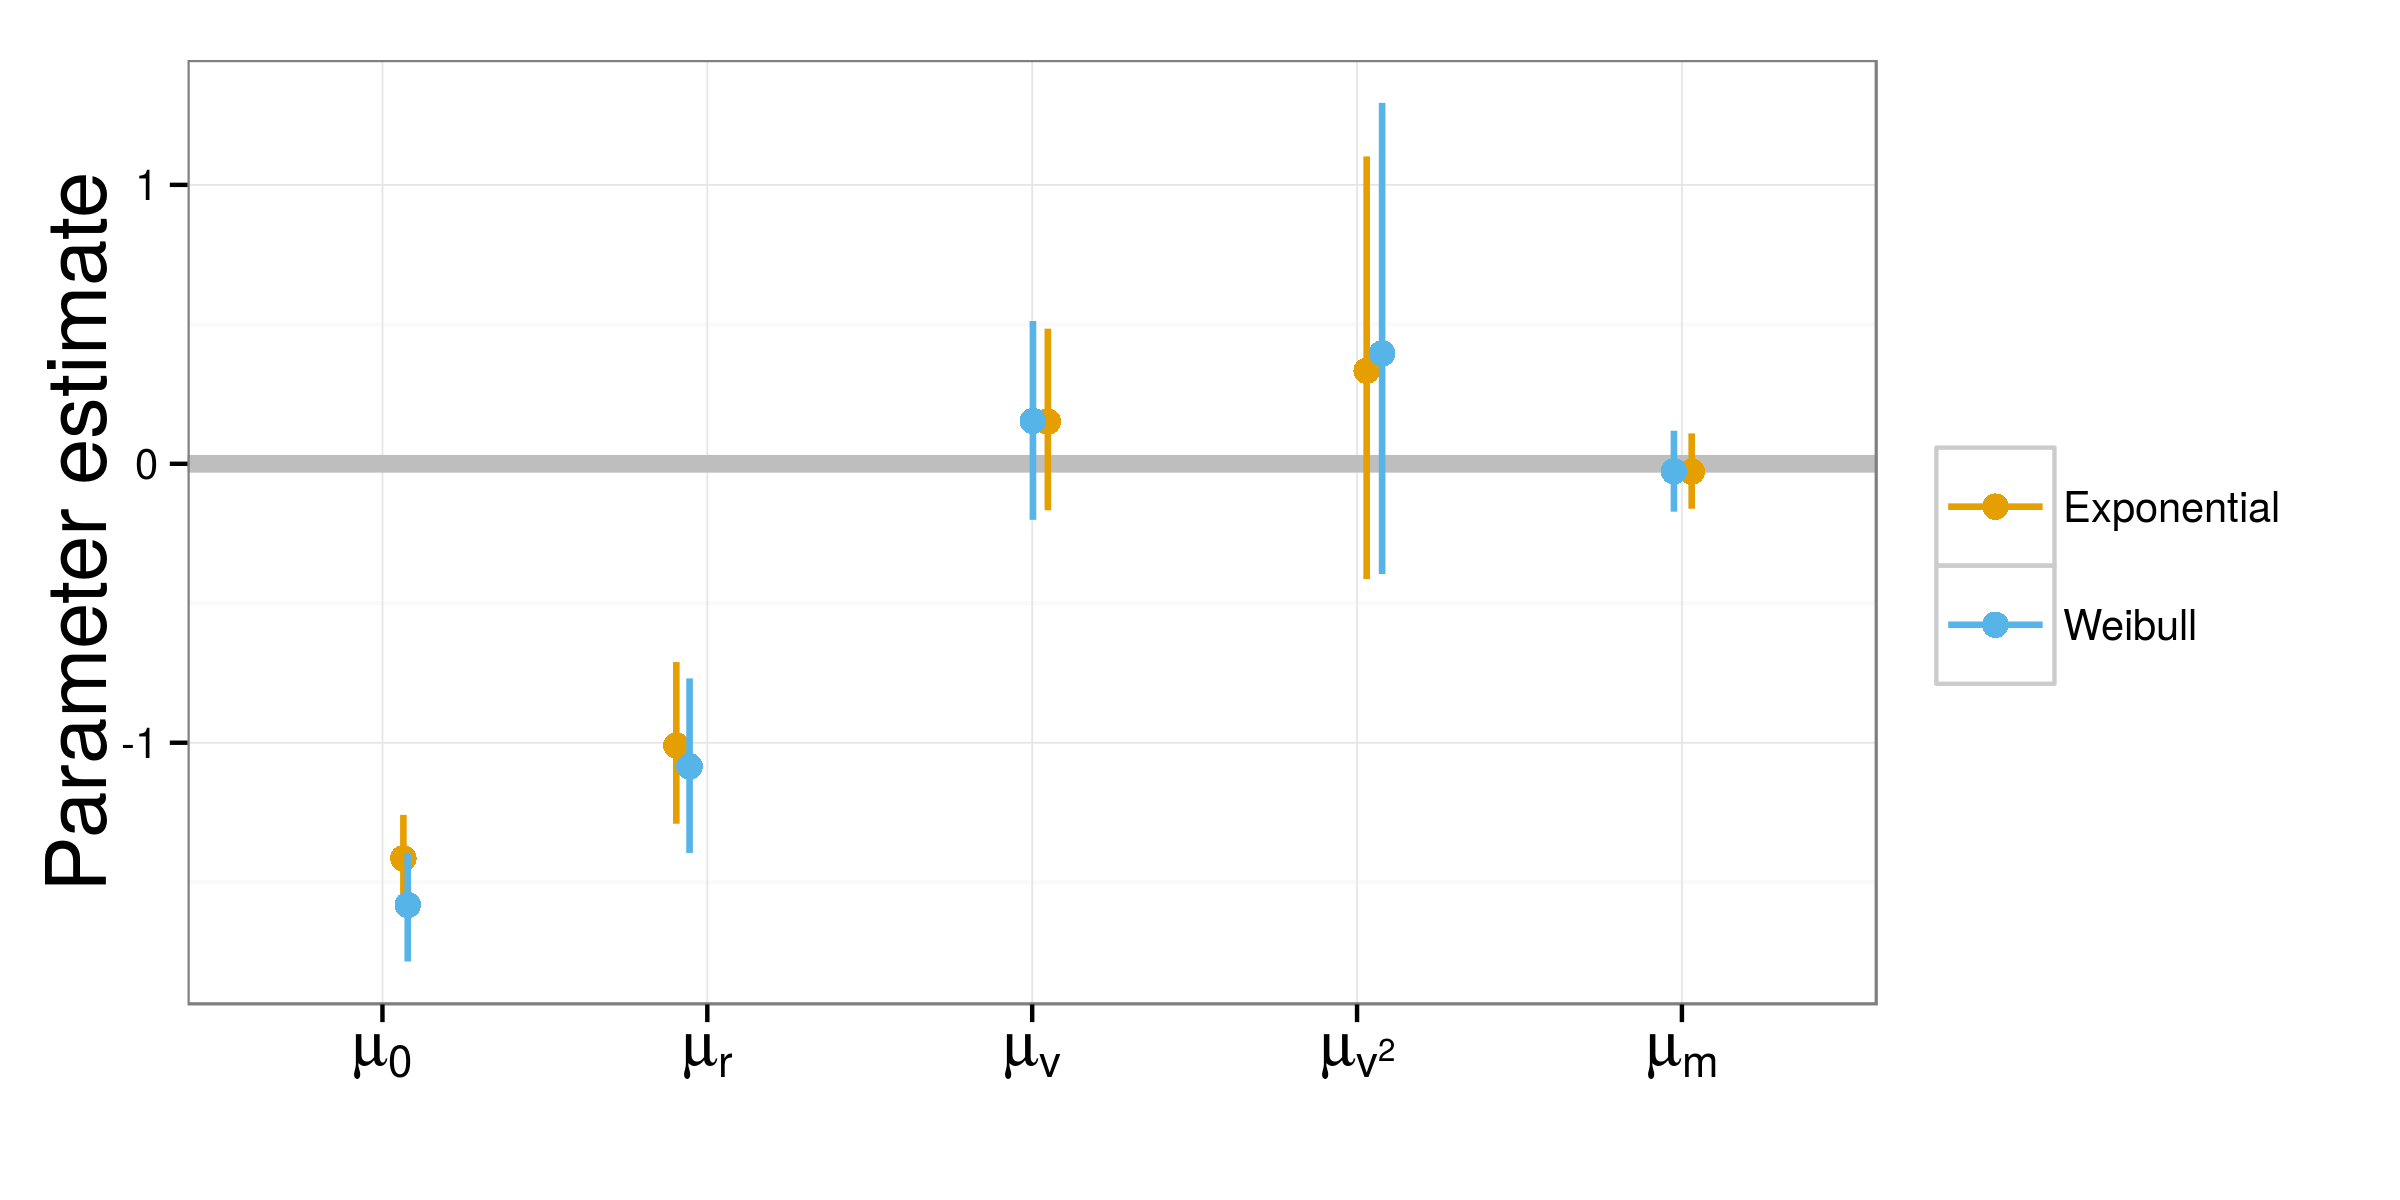
\includegraphics[height = 0.5\textheight,width=\textwidth,keepaspectratio=true]{figure/coef_means}
  \caption{<+caption text+>}
  \label{fig:mu}
\end{figure}

Interpretation of the effect of environmental preference \(v\) on duration is slightly more involved. Because a quadratic term is the equivalent of an interaction term, both \(\mu_{v}\) and \(\mu_{v^{2}}\) have to be interpreted together because it is illogical to change values of \(v\) and only affect one of the coefficients. To determine the nature of the effect of \(v\) on duration I calculated the multiplicative effect of environmental preference on extinction risk.

Given mean estimated extinction risk \(\tilde{\sigma}\), we can define the extinction risk multiplier of an observation with environmental preference \(v_{i}\) as 
\begin{equation}
  \frac{\tilde{\sigma_{i}}}{\tilde{\sigma}} = \exp\left(\frac{-(\mu_{v} v_{i} + \mu_{v^{2}} v^{2})}{\alpha}\right).
  \label{eq:env}
\end{equation}
This exponentiated quadratic function has a y-intercept of \(\log(0)\) or 1 by definition. Equation \ref{eq:env} can be either upward or downward facing. A downward facing function indicates that genera of intermediate environmental preference have greater durations than either extreme, and \textit{vice versa} for upward facing functions.

The estimated mean effect of environmental preference as a multiplier of mean extinction risk can then be simply visualized (Fig. \ref{fig:env_mean}). This figure depicts 1000 posterior predictive estimates of Eq. \ref{eq:env} across all possible values of \(v\). The number indicates the posterior probability that the function is downward facing, with generalists having lower extinction risk/greater duration than either type of specialist. Note that the inflection point/optimum of Fig. \ref{fig:env_mean} is at approximately 0, something that is observable given the estimate of \(\mu_{v}\) (Fig. \ref{fig:mu}).
\begin{figure}[ht]
  \centering
  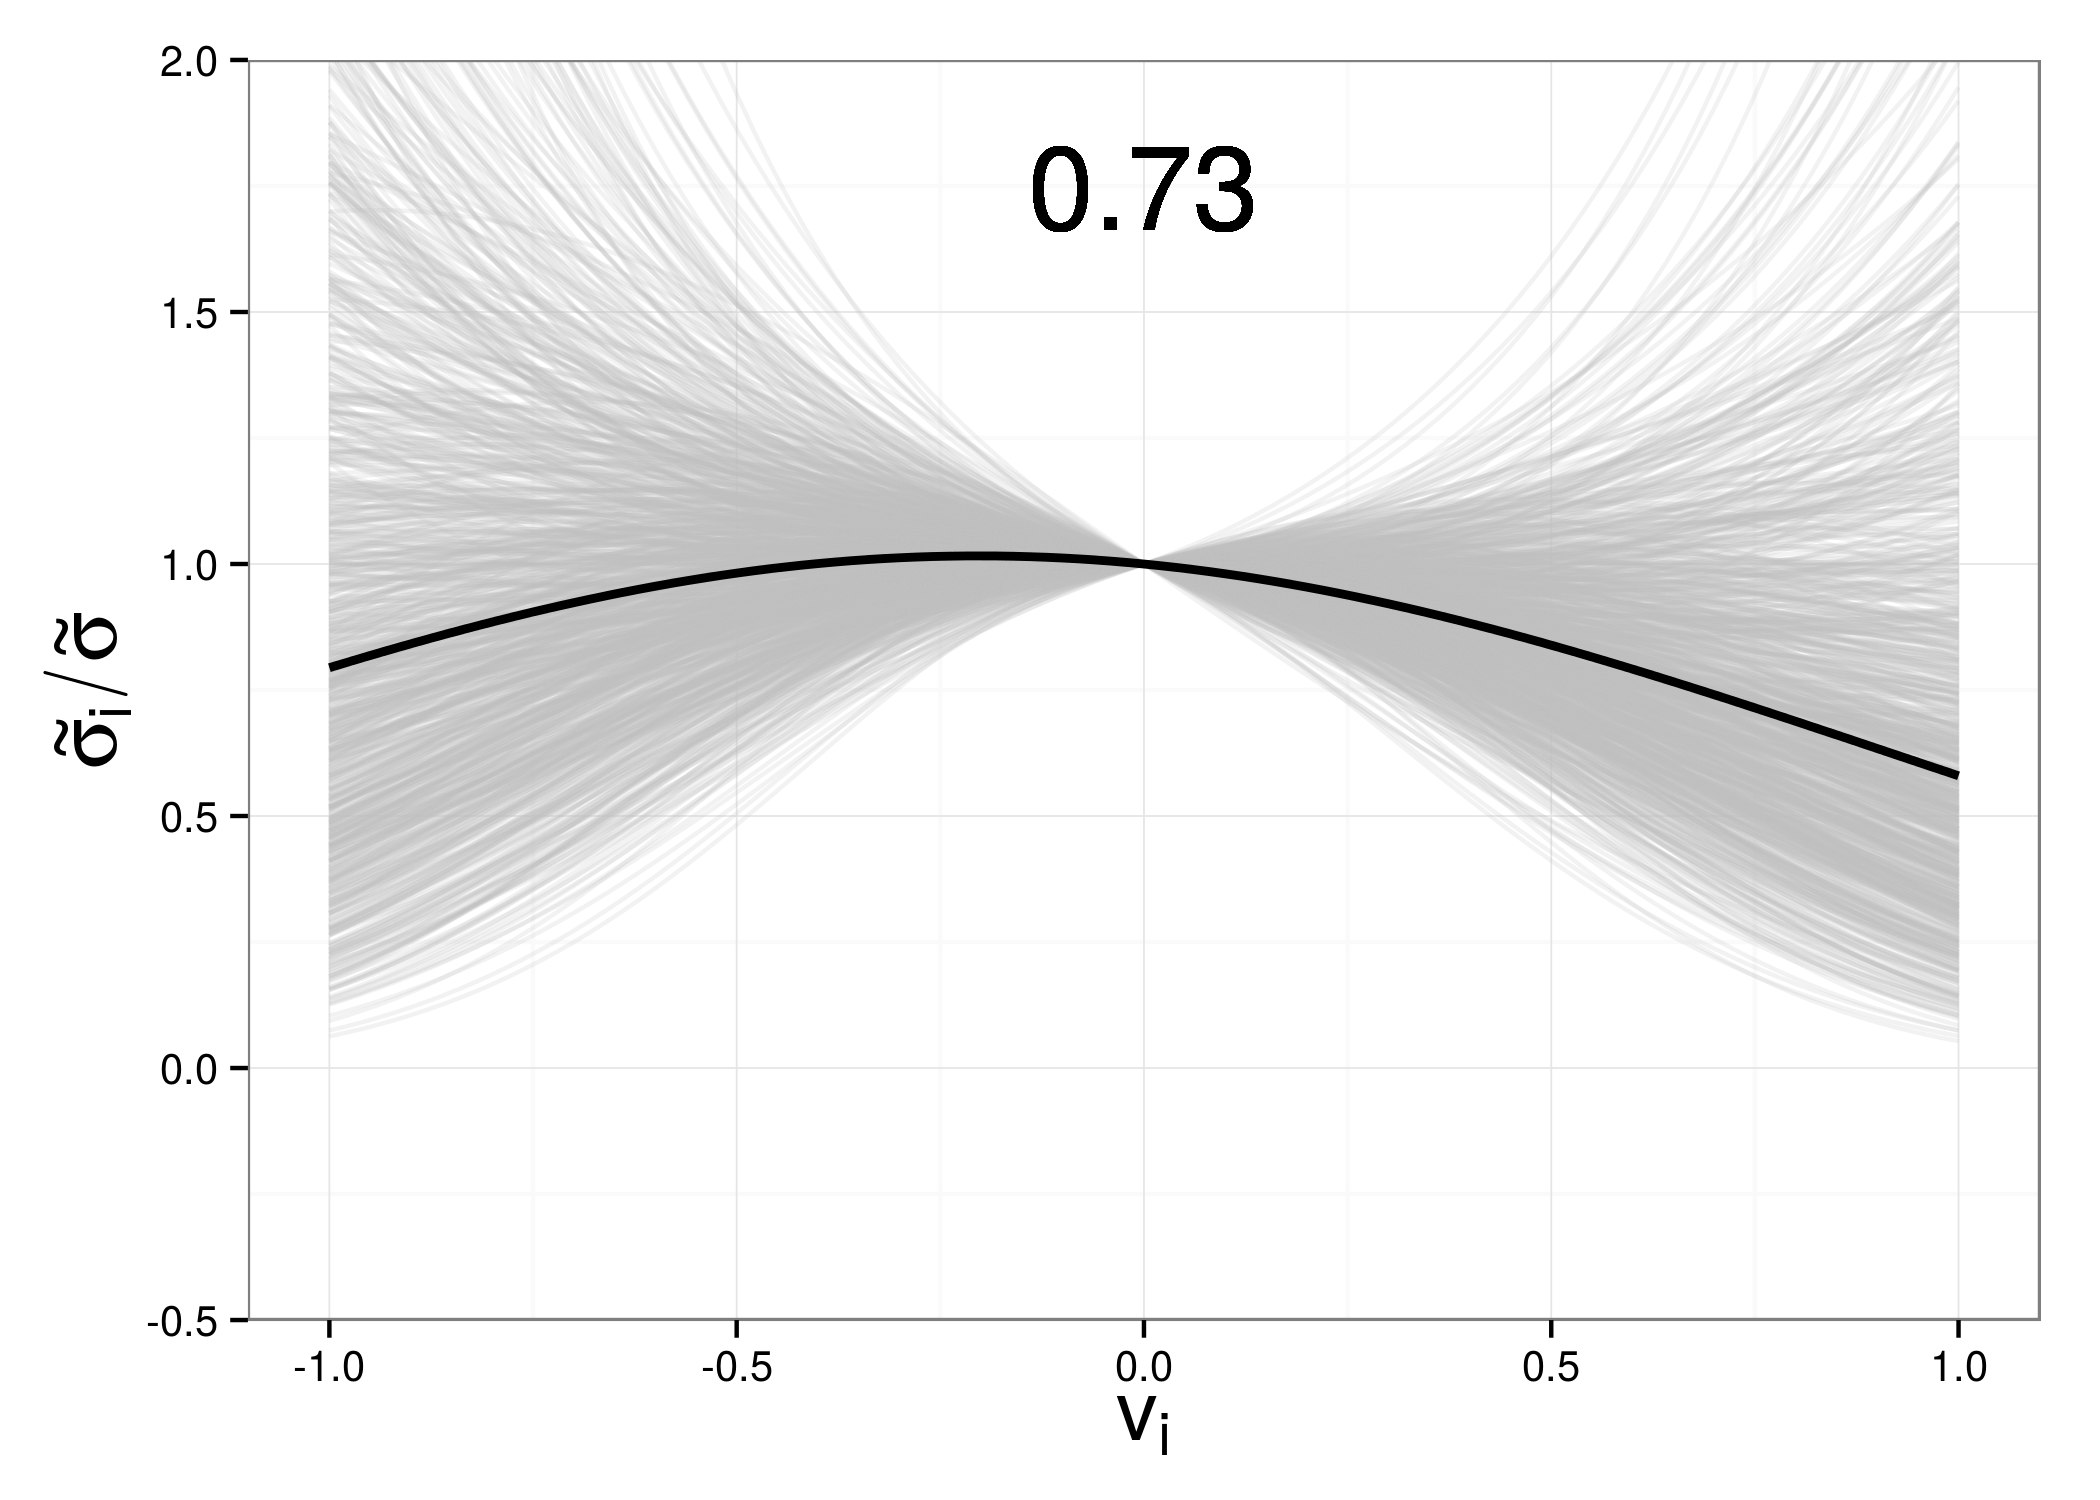
\includegraphics[height = 0.5\textheight,width=\textwidth,keepaspectratio=true]{figure/environ_quad}
  \caption{<+caption text+>}
  \label{fig:env_mean}
\end{figure}

The matrix \(\Sigma\) describing the covariance between the different coefficients describes how these coefficients might vary together across the origination cohorts. Similar to how this was modeled (Eq. \ref{eq:exp_total}, \ref{eq:wei_total}), \(\Sigma\) can be decomposed into a vector of standard deviations \(\tau\) and a correlation matrix \(\Omega\).

The estimates of the standard deviation of between cohort coefficient estimates \(\tau_{B}\) vary greatly (Fig. \ref{fig:tau}). Coefficients with greater values of \(\tau\) have greater between cohort variation. The covariate effect with the greatest between origination cohort variation is \(\beta_{v^{2}}\) with \(\beta_{r}\) being the second largest. Both \(\beta_{v}\) and \(\beta_{m}\) have little between cohort variation, as both have less variation than mean extinction risk \(\beta_{0}\). However the amount between cohort variation in estimates of \(\beta_{v}\) means that it is possible that the function describing the effect of environment can be upward facing for some cohorts (Eq. \ref{eq:env}), meaning that environmental generalists being shorted lived than specialists.
\begin{figure}[ht]
  \centering
  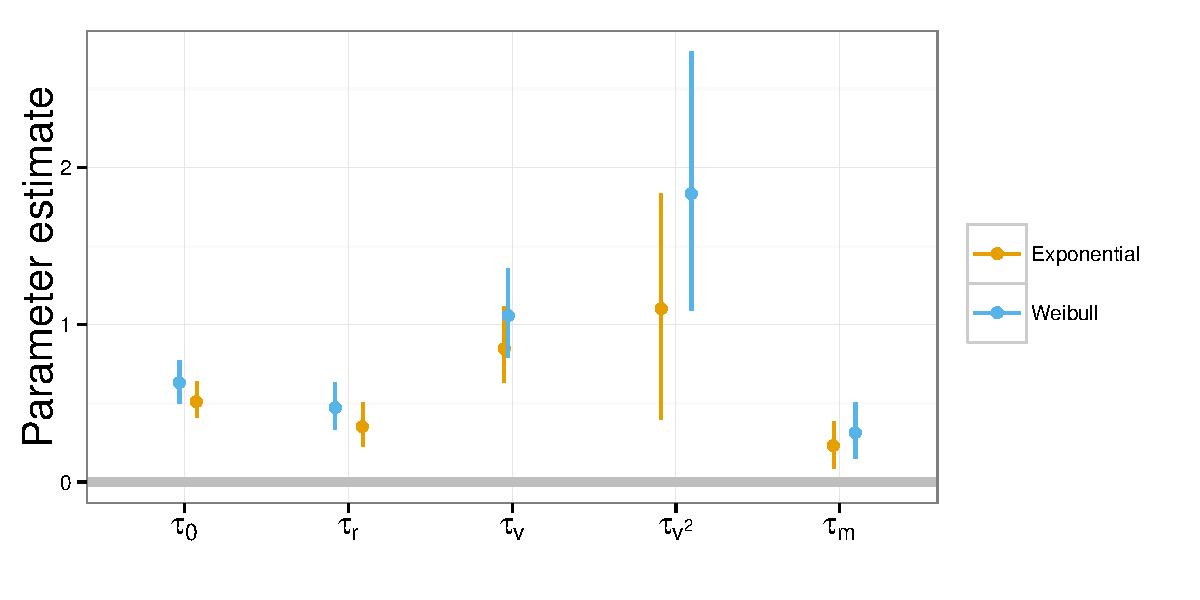
\includegraphics[height = 0.5\textheight,width=\textwidth,keepaspectratio=true]{figure/coef_var}
  \caption{<+caption text+>}
  \label{fig:tau}
\end{figure}


% omega heatmap
%   correlations with baseline extinction risk of of major interest
%   high/positive values of intercept --> high extinction risk
%   low/negative values of intercept --> low extinction risk
The correlation matrix \(\Omega\) shows a few important correlations between the coefficients (Fig. \ref{fig:omega}). The correlation terms describe the relationship between the coefficients and how their estimates may vary together across cohorts. Of particular note are the correlations between the intercept term \(\beta_{0}\), or expected extinction risk, and the biological covariates (Fig. \ref{fig:omega} first column/last row). Keep in mind that when \(\beta_{0}\) is low, extinction risk is low; and conversely, when \(\beta_{0}\) is high, then extinction risk is high.
\begin{figure}[ht]
  \centering
  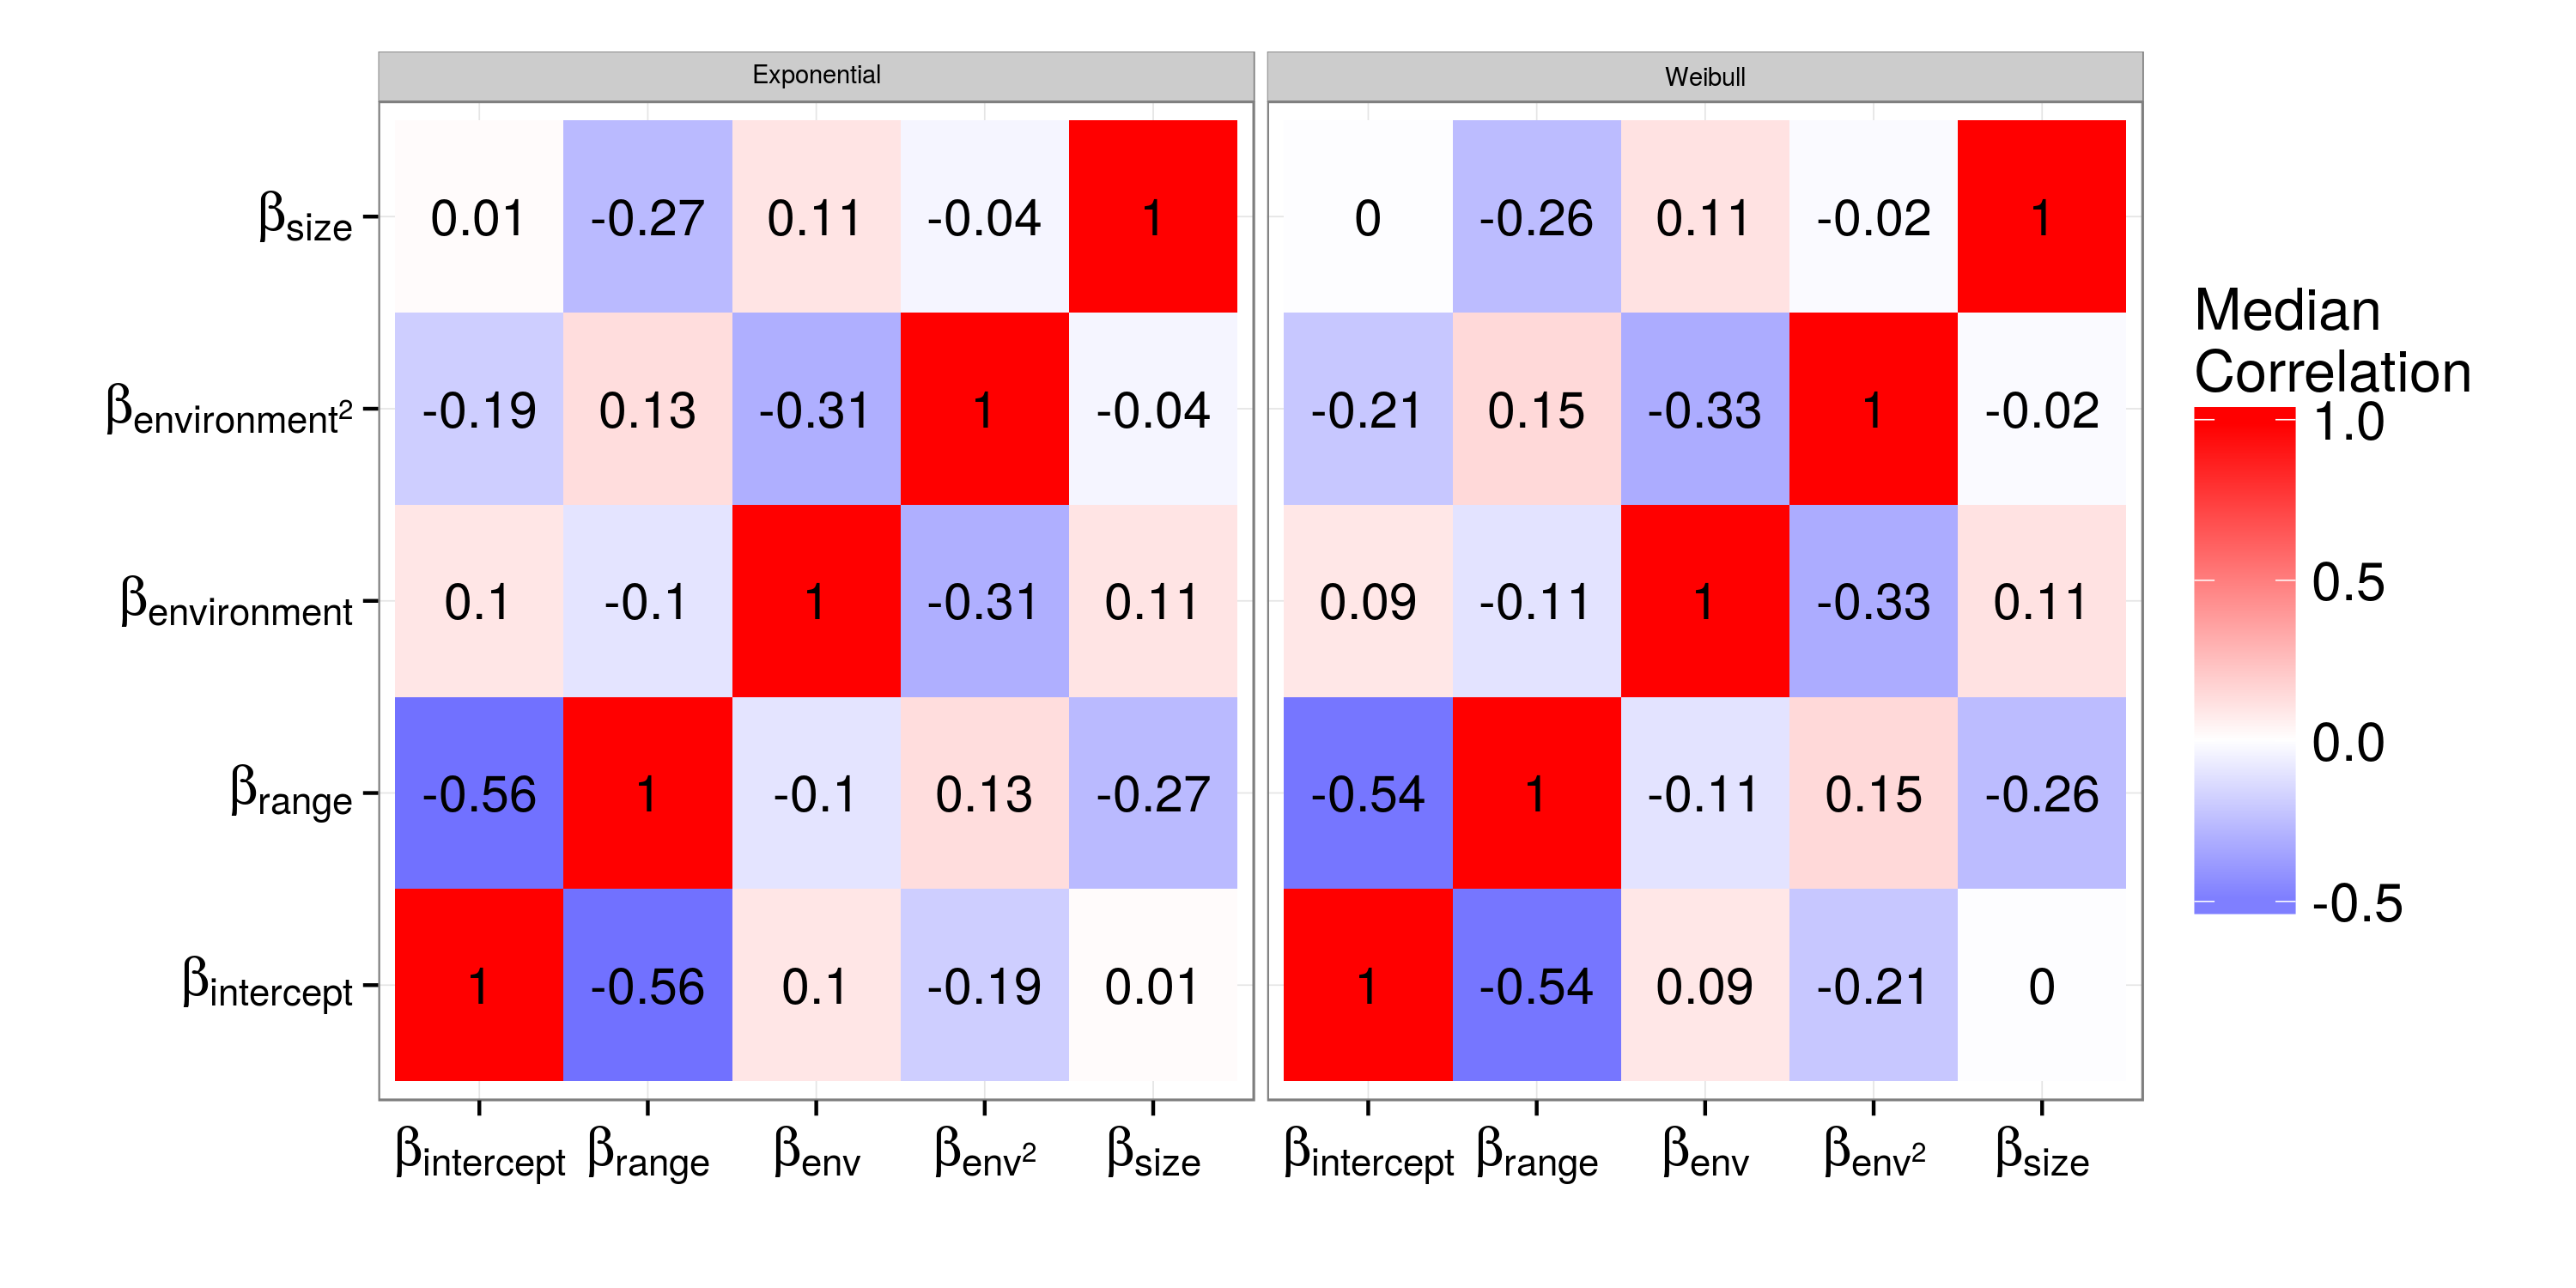
\includegraphics[height = 0.5\textheight,width=\textwidth,keepaspectratio=true]{figure/correlation_heatmap}
  \caption{<+caption text+>}
  \label{fig:omega}
\end{figure}

The marginal posterior estimates for the correlations between estimates of the \(\beta_{0}\) and the effects of the biological covariates indicate that the relationships between expected extinction risk and either geographic range \(\beta_{r}\) is of note (Fig. \ref{fig:corr}). The negative correlation between \(\beta_{0}\) and \(\beta_{r}\) implies that as extinction risk increases, the effect/importance of geographic range on genus duration increases. %Similarly, the correlation between \(\beta_{0}\) and \(\beta_{v^{2}}\) implies that as extinction risk increases, the function describing the effect of environmental preference flattens (and potentially inverts).
\begin{figure}[ht]
  \centering
  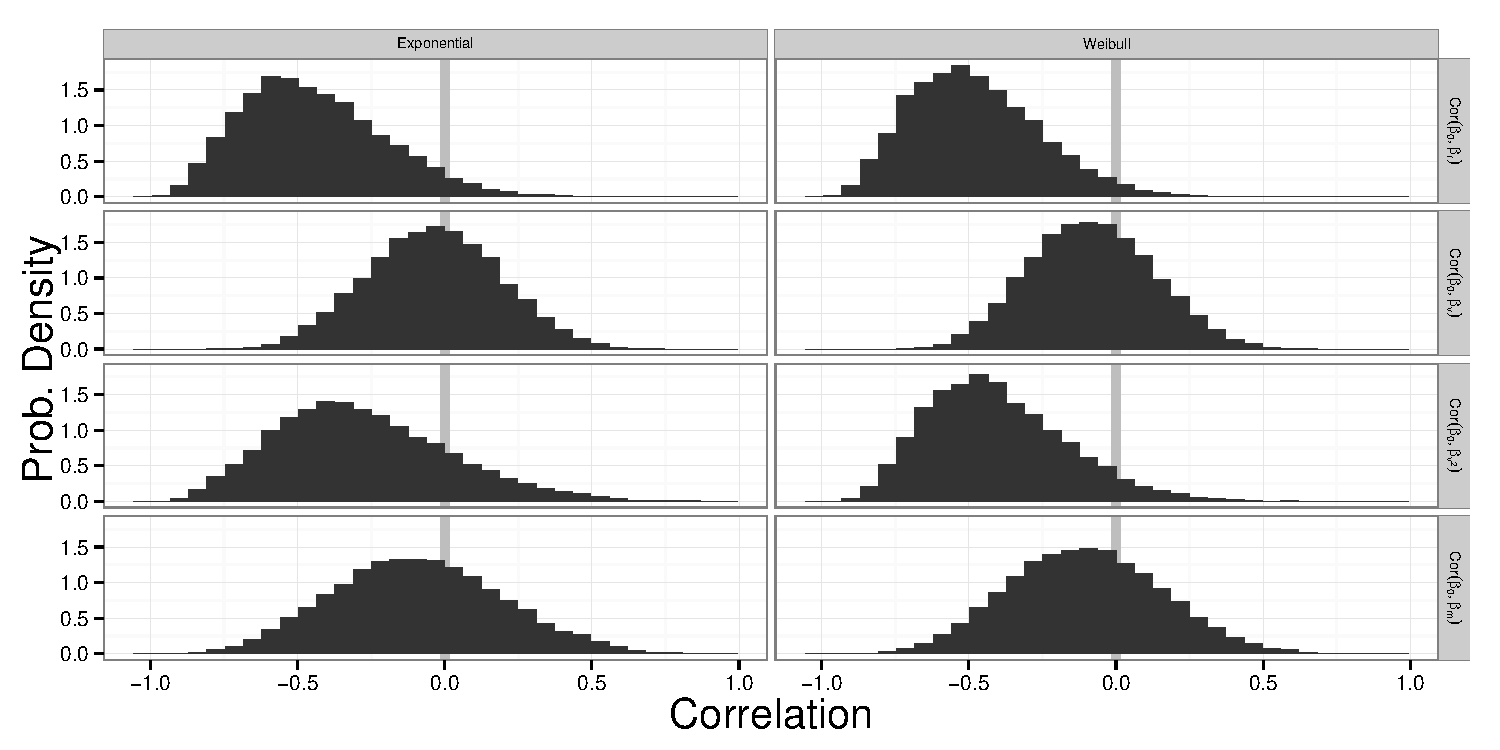
\includegraphics[height = 0.5\textheight,width=\textwidth,keepaspectratio=true]{figure/correlation_marginal}
  \caption{<+caption text+>}
  \label{fig:corr}
\end{figure}

% effects varying between cohorts
In addition to just analyzing the covariance matrix between the coefficient estimates, it is important to also observe the individual origination cohort level estimates. 

In comparison to the overall mean extinction risk \(\mu_{intercept}\), cohort level estimates \(\beta_{0}\) show some amount of variation through time as expected by estimates of \(\tau_{intercept}\) (Fig. \ref{fig:cohort_intercept}). A similar, if slightly greater, amount of variation is also observable in cohort estimates of the effect of geographic range \(\beta_{0}\) (Fig. \ref{fig:cohort_range}). Again, smaller values of \(\beta_{0}\) correspond to lower expected extinction risk. Similarly, smaller values of \(\beta_{0}\) correspond to greater decrease in extinction risk with increasing geographic range 
\begin{figure}[ht]
  \centering
  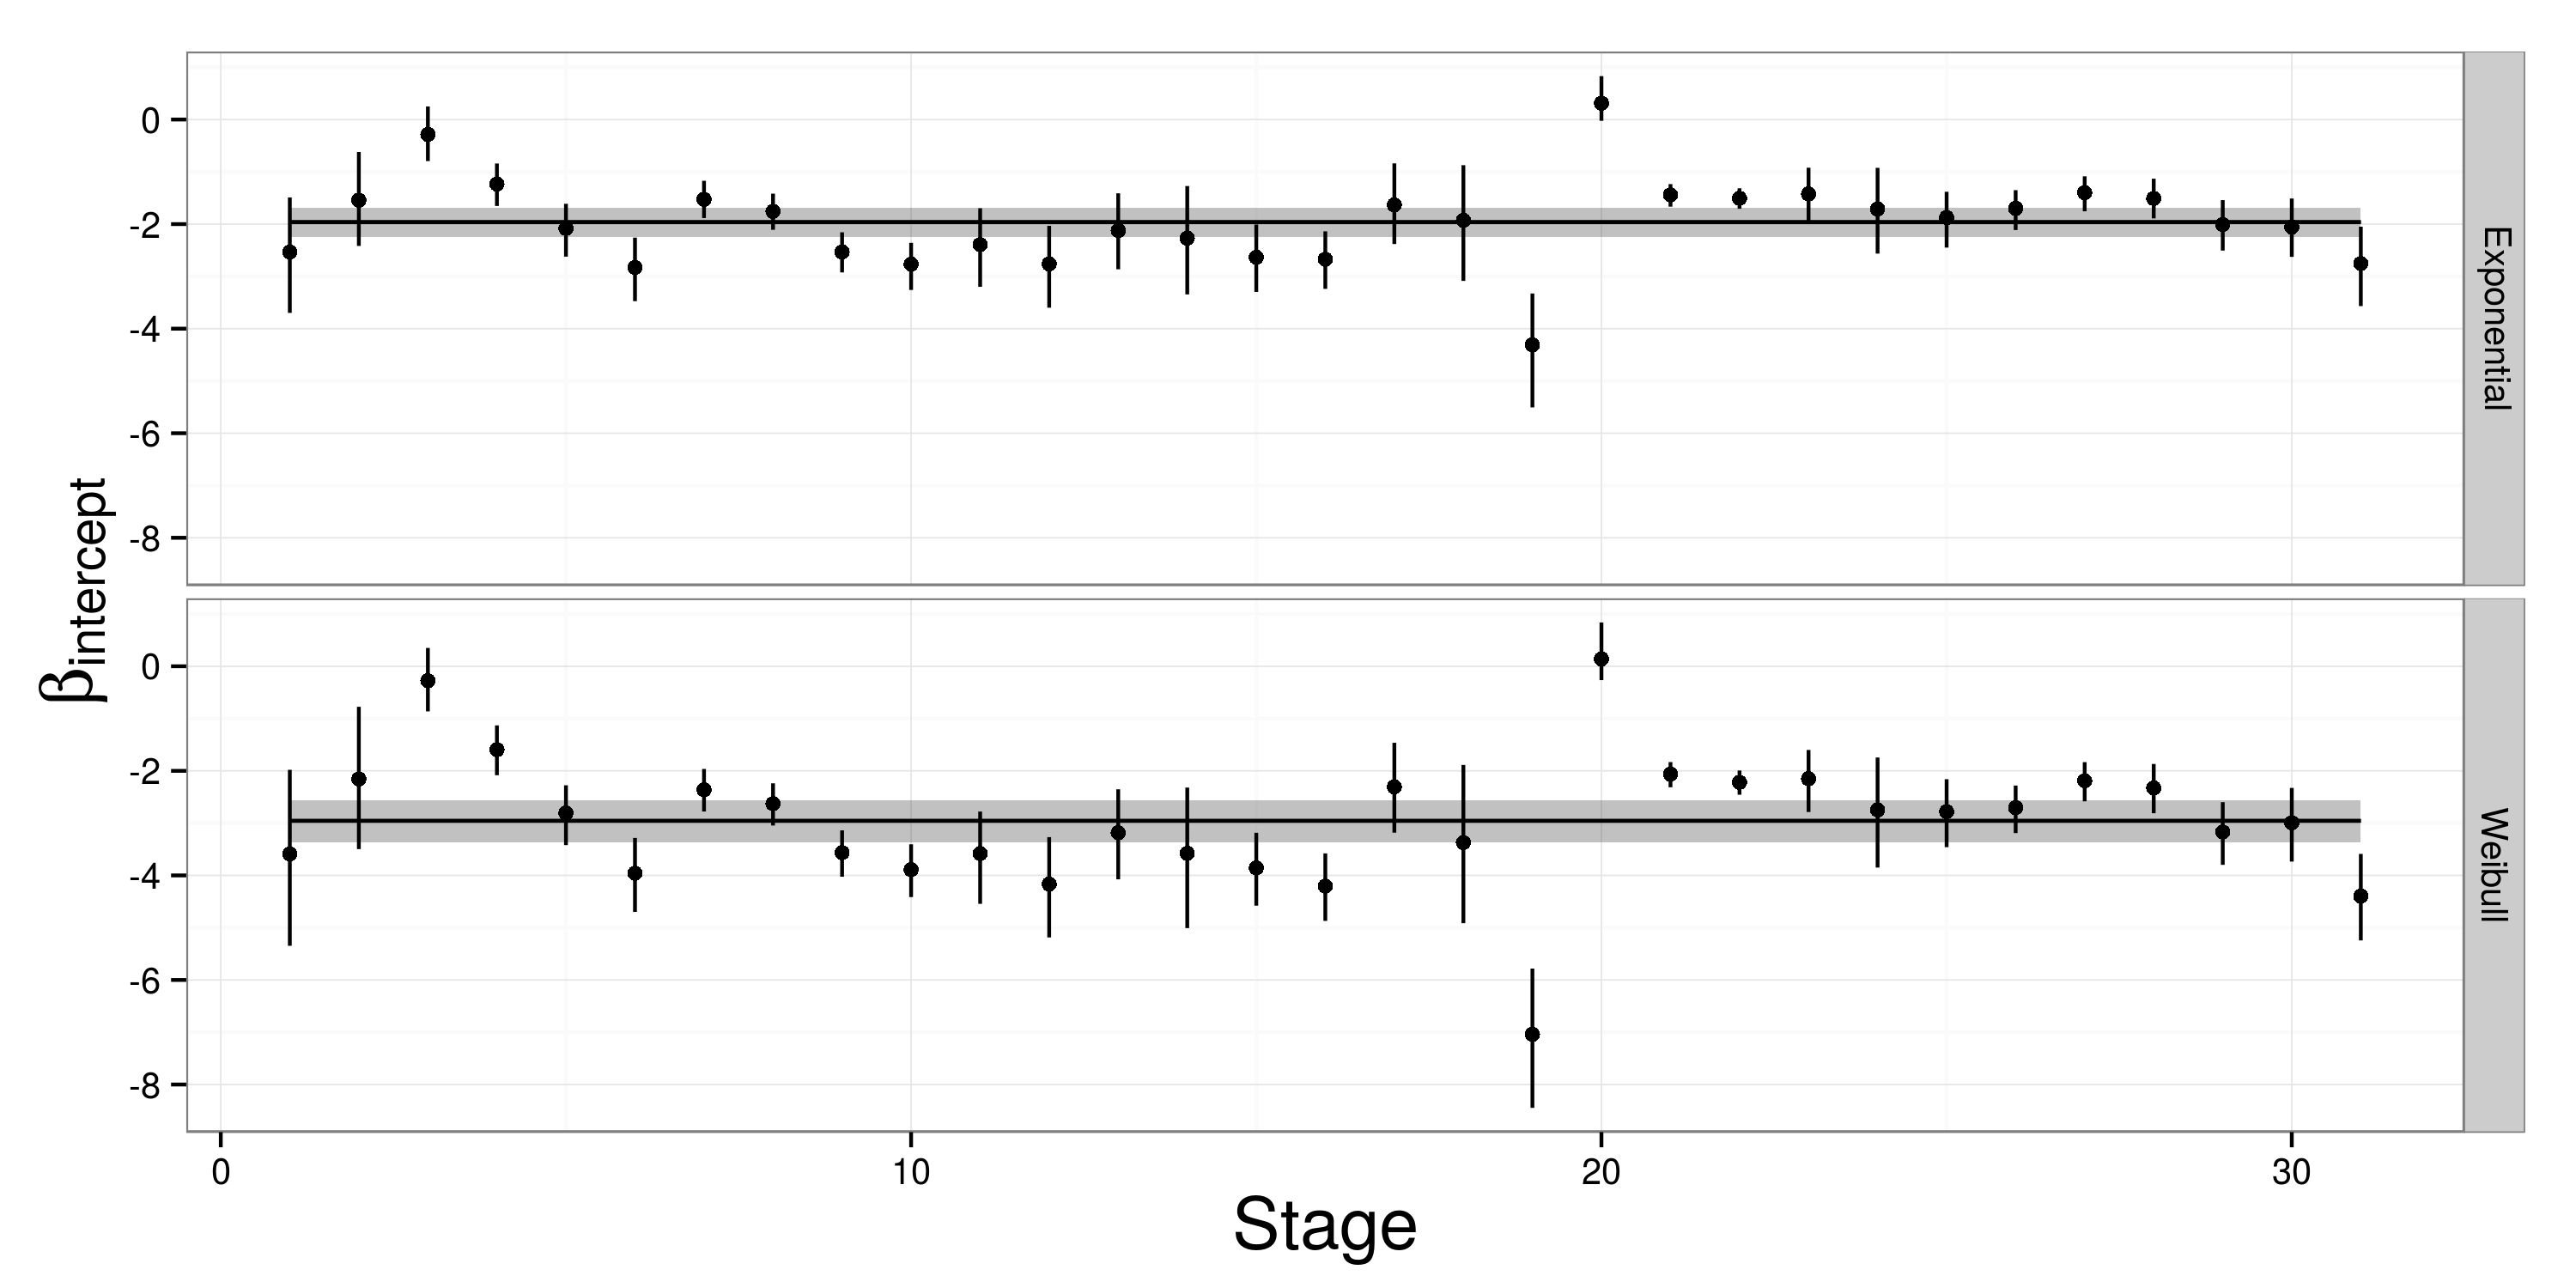
\includegraphics[height = 0.5\textheight,width=\textwidth,keepaspectratio=true]{figure/intercept_cohort}
  \caption{<+caption text+>}
  \label{fig:cohort_intercept}
\end{figure}

\begin{figure}[ht]
  \centering
  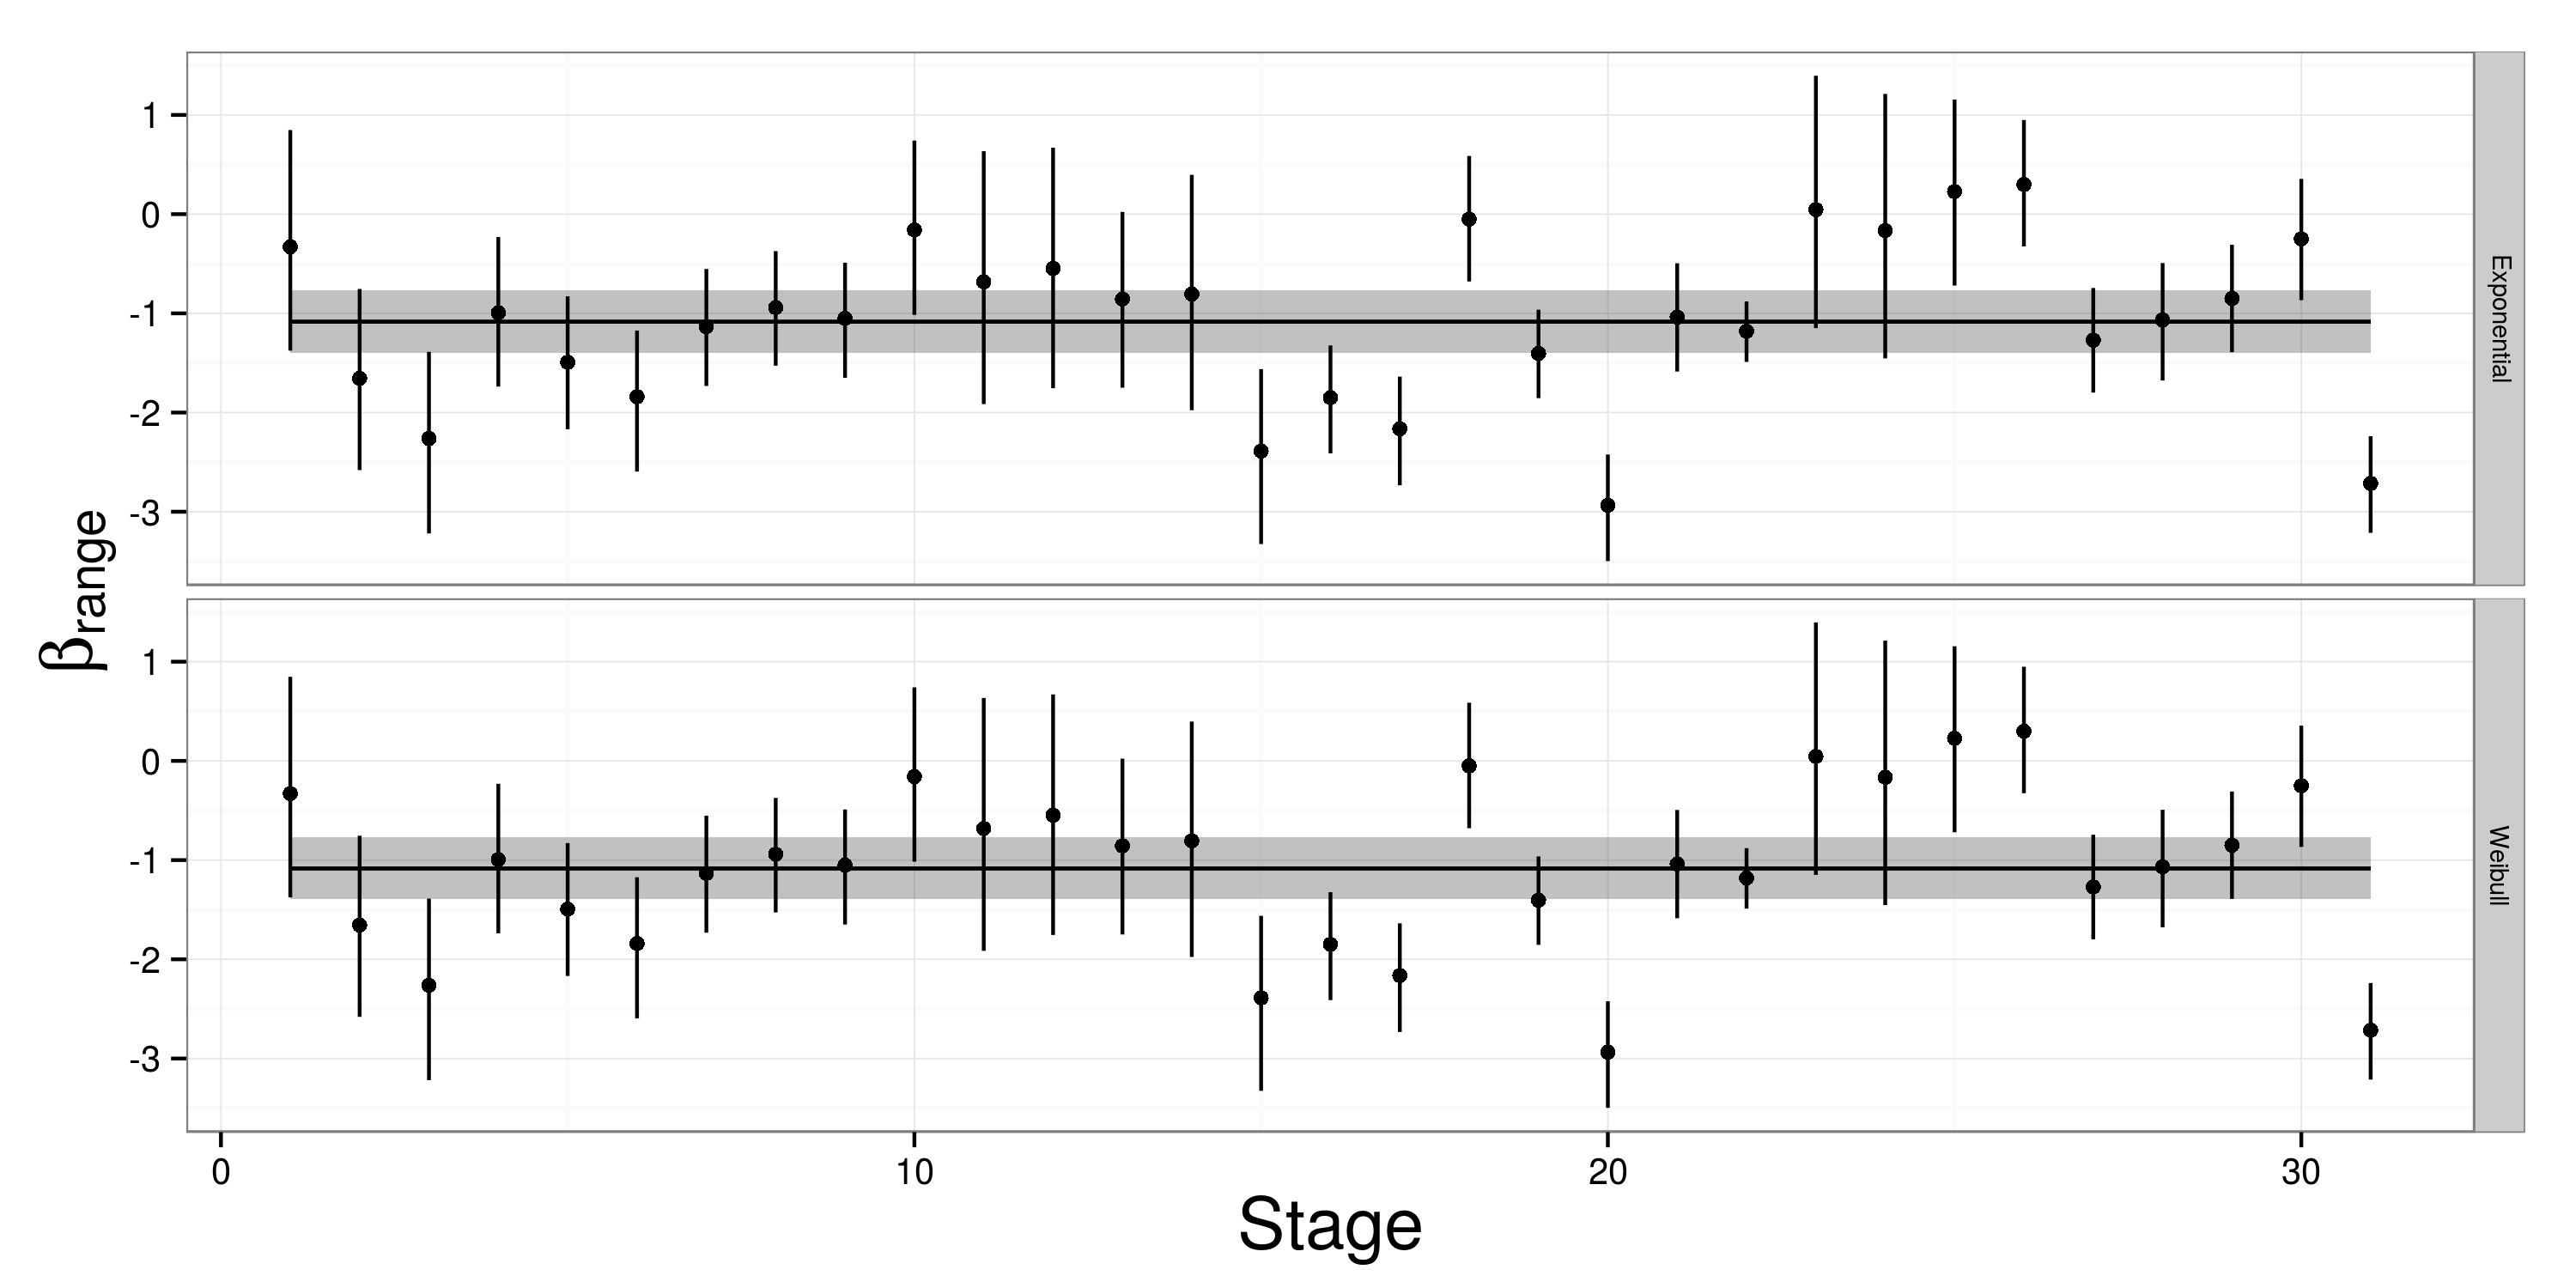
\includegraphics[height = 0.5\textheight,width=\textwidth,keepaspectratio=true]{figure/range_cohort}
  \caption{<+caption text+>}
  \label{fig:cohort_range}
\end{figure}

% environmental effect for cohort
%   effect of environmental preference as duration multiplier
How environmental effect varies between cohorts can be observed by using the cohort specific estimates of the coefficients \(\mathbf{B}_{j}\). Following the exact same procedure for generating figure \ref{fig:tau}, but substituting \(\beta_{v; j}\) and \(\beta_{v^{2}; j}\) for \(\mu_{v}\) and \(\mu_{v^{2}}\), the cohort specific effect of environmental preference as a multiplier of mean extinction risk can be calculated. This was done only for the Weibull model, though the observed pattern should be similar for the exponential model. 

As expected based on the estimates of \(\tau_{v}\) and \(\tau_{v^{2}}\), there is greater variation in the peakedness of the function than there is variation between upward and downward facing functions (Fig. \ref{fig:env_cohort}. Only 9 of the 31 cohorts have less than 50\% posterior probability that generalists are shorter lived than specialists, though 2 of those cases have approximately a 50\% probability of being either upward or downward facing. This is congruent with the 0.70+ posterior probability that \(\mu_{v^{2}}\) is positive/the relationship is downward facing, which corresponds to approximately 8 out of 31 cohorts.

Additionally, a quite striking pattern emerges when the inflection point of the function is either far away from the y-intercept (x = 0, y = 1) or when there is little evidence non-linearity (Fig. \ref{fig:env_cohort}). Cohort 21 and 20, for example, have almost linear relationships between environmental preference and duration multiplier. This type of relationship occurs when \(\beta_{v^{2}}\) approaches 0, flattening the non-linear curvature of the relationship.

\begin{sidewaysfigure}[ht]
  \centering
  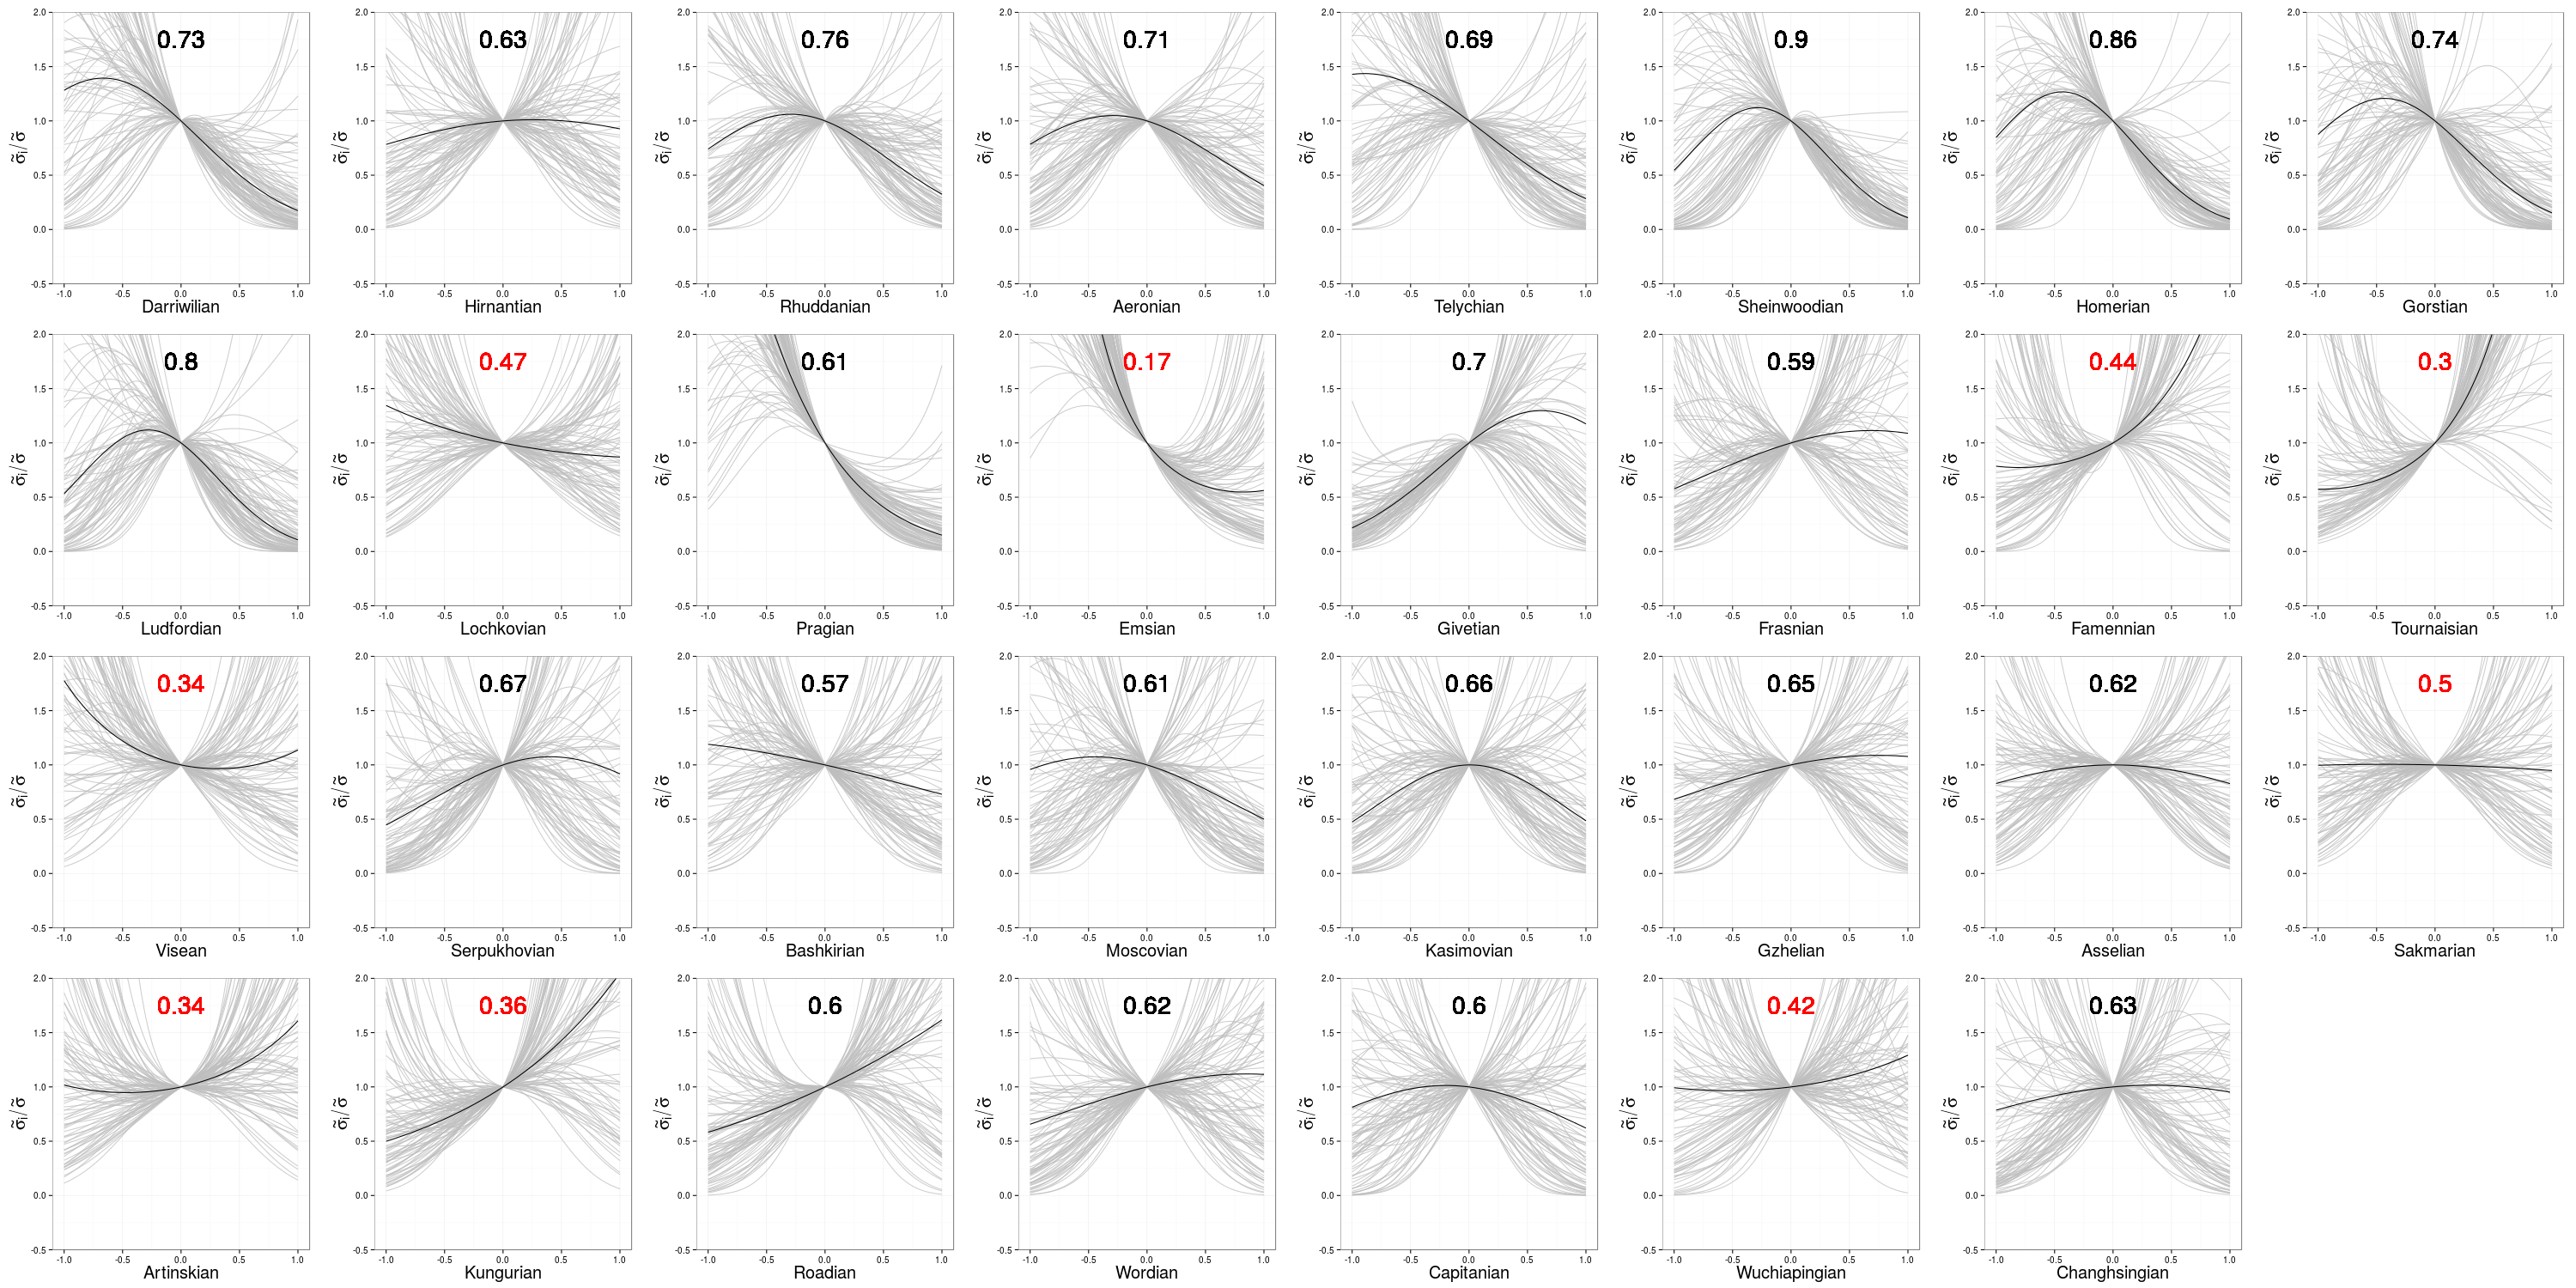
\includegraphics[height = 0.5\textheight,width=\textwidth,keepaspectratio=true]{figure/cohort_quads}
  \caption{<+caption text+>}
  \label{fig:env_cohort}
\end{sidewaysfigure}


\end{document}
